\documentclass[12pt]{article}

\usepackage{graphicx}
\graphicspath{ {../plots/} }
\usepackage{caption}
\usepackage{subfigure}

\usepackage[%
  backend=bibtex      % biber or bibtex
 ,style=authoryear-ibid
 ,sorting=none
 , dashed=false
]{biblatex}
\addbibresource{bib_file.bib}
\DeclareNameAlias{sortname}{first-last}


\title{Traffic Accidents Analysis}
\date{}

\begin{document}

\maketitle


% ANALYSIS

\section{Introduction}

The following report is an analysis of traffic accidents in the United Kingdom during the year of 2019, based on the freely available data published by the Department for \parencite{accidents2019, vehicles2019, casualties2019}. There are two primary concerns of traffic accidents, the frequency at which they occur and their severity. As such, the report will focus on those metrics.

The report is structured as follows. Firstly, a broad, frequentist approach to find common trends in the data, followed by the testing of three distinct hypotheses. Next, a probabilistic model was developed to predict the severity of accidents based on a subset of the predictors that are recorded via \textcite{stats2019}. Finally, a selection of recommendations are proposed with reference to the analysis performed.

\section{Analysis}

\subsection{Data Cleaning}

The data employed in this analysis was for the most part clean and structured, except for a few key areas.

There were twenty-eight samples with missing coordinate data. However, these samples did have associated local district information. By use of the Beautiful Soup package \parencite{bs4}, the coordinate data from all towns and cities in the United Kingdom were scraped from \cite{cities} and imputed into the dataset where coordinate data was lacking.

A similar approach was taken to impute missing time values. In this case, the sunrise and sunset times for London were scraped from the web \parencite{sunrise_sunset}. According to the light conditions of the sample, the median time between sunrise and sunset on the day of the accident was imputed in the case of light, and the median time between sunset and sunrise in the case of darkness. The purpose of this was to ensure that imputed data does not contradict the obvious and empirically true covariance between the time of the day and light conditions.

\subsection{Primary Analysis}

\subsubsection{Geospaital Analysis}

An initial clustering analysis based around eight cluster centres shows that generally the vast majority of accidents occur in densely populated areas, with significant levels in London, Birmingham, Manchester, Leeds, Newcastle and Edinburgh. However, it can also be seen that there is a significant number of accidents in Wales and in the South East, which would suggest that accidents also occur frequently in rural areas. Based on this result, the hypothesis regarding accidents in rural locations was carried out.

\begin{figure}[ht]
\centering     %%% not \center
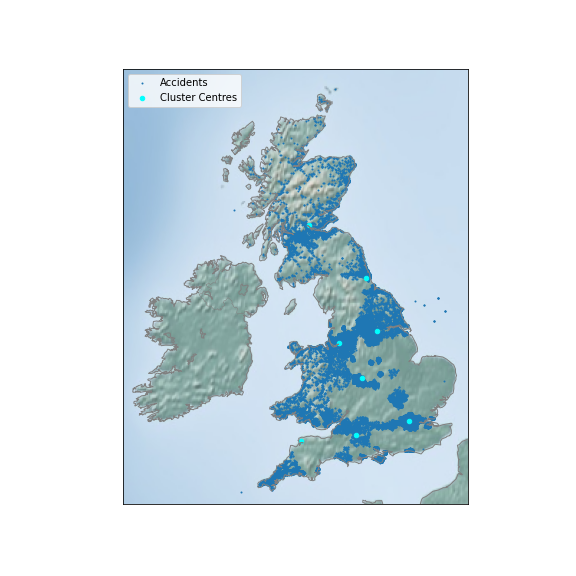
\includegraphics[width=0.70\textwidth]{accident_clusters}
\caption{Geospatial clustering of accidents.}
\end{figure}

\newpage

\subsubsection{Temporal Analysis}

Considering the temporal dimension of the data, it was determined that there exist two primary peaks in accident frequency within the ranges 8am-10am, and then again from 3pm to 7pm, shown in figure \ref{fig:a-hour_of_day}.

\begin{figure}[h]
\centering     %%% not \center
\subfigure[Accidents by time of day.]{\label{fig:a-hour_of_day}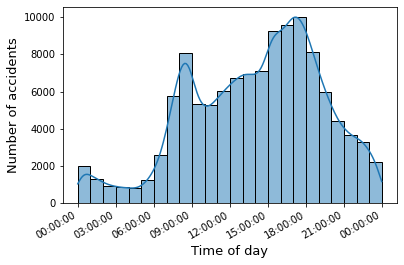
\includegraphics[width=0.45\textwidth]{time_of_day}}
\subfigure[Accidents by day of the week.]{\label{fig:b-day_of_week}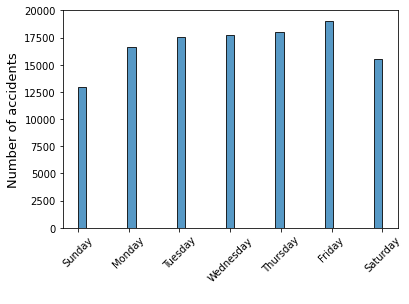
\includegraphics[width=0.45\textwidth]{day_of_week}}
\caption{Temporal analysis of accident frequency.}
\end{figure}

These are the usual times at which people commute, and so such increases are to be expected.

Further, it can be seen from figure \ref{fig:b-day_of_week} that the frequency of traffic accidents is generally higher during the weekdays, with the maximum on Friday and the minimum on Sunday. This further supports the hypothesis that there is a significant increase in accidents during work-commute periods.

\subsubsection{Vehicle Types}

In the next stage of analysis, the aggregated accident data was partitioned according to the type of vehicle.

Both the absolute number of accidents, as well as the proportion of total accidents was considered on the temporal axis, as can be seen in figure \ref{vehicles-day-week}.

There is accident data for a total of twenty vehicle classifications. To simplify the analysis, only those contributing more than 2\% of the total number of accidents were considered.

\begin{figure}[h]
\centering     %%% not \center
\subfigure[Vehicle type by time of day.]{\label{fig:a-vehicle-hour}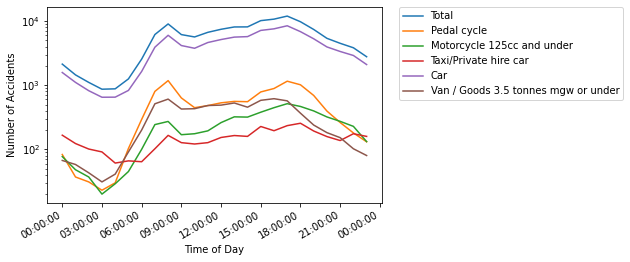
\includegraphics[width=0.80\textwidth]{vehicle_hour_plot}}
\subfigure[Vehicle type by day of the week.]{\label{fig:b-vehicle-day}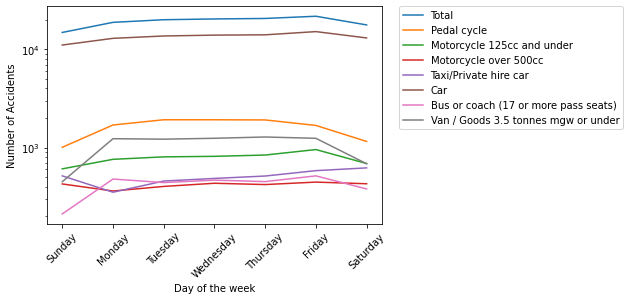
\includegraphics[width=0.80\textwidth]{vehicle_day_plot}}
\caption{Type of vehicle involved in accidents.}
\label{vehicles-day-week}
\end{figure}

\newpage

As can be seen from \ref{fig:a-vehicle-hour}, the distribution of accidents for each vehicle type generally follows the overall distribution for time of day. The one exception is for taxis and private car hire, which has a higher relative frequency of accidents between midnight and 9:00am than other vehicle types.

\newpage

\subsection{Hypothesis Testing}

The following section describes three hypotheses that have been tested. The hypotheses are as follows:

\begin{itemize}
\item Is there a significant number of accidents in rural areas caused by or involving drivers who do not live in the vicinity, and which type of vehicles are involved?
\item Is there more accidents at the same time of day during periods of the year after which the sun has gone down compared to when it is still light?
\item Is there more accidents in the vicinity of football grounds on days when premier league football matches take place?
\end{itemize}

\subsubsection{Rural Accidents}

To test this hypothesis the data was filtered for the conjunction of accidents taking place in rural areas and drivers who do not live in rural areas. 

\begin{figure}[h]
\centering     %%% not \center
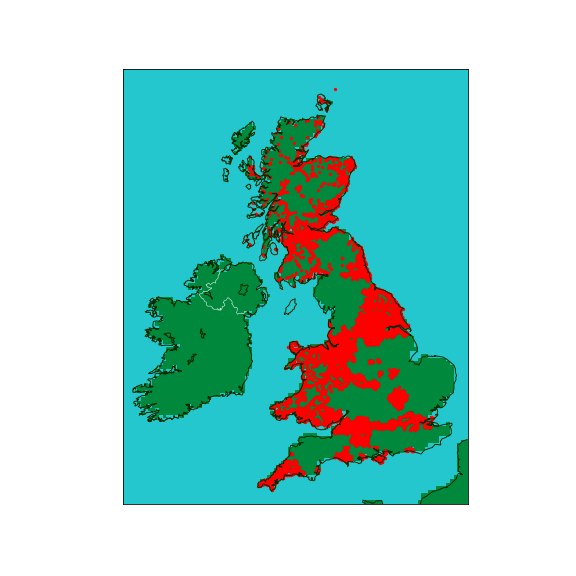
\includegraphics[width=0.70\textwidth]{rural_accidents}
\caption{Accidents in rural areas caused by people not living in rural areas.}
\label{rural-uk}
\end{figure}

As shown in figure \ref{rural-uk}, by plotting the geospatial data for this subset, it can be seen that a significant number of accidents occurring in rural areas of Wales, the South East, North Yorkshire and Scotland are caused by people who do not live in such areas.

\newpage

Next, we determined the ratio of accidents in rural areas involving people not living in those areas to the total frequency of accidents, parametrised by vehicle type, figure \ref{vehicle-rural}.

Hence, we see that the most significant increase in accidents in rural areas exist for motorcyclists of 500cc and higher, horse riders and mobility scooter riders.

\newpage

\begin{figure}[h]
\centering     %%% not \center
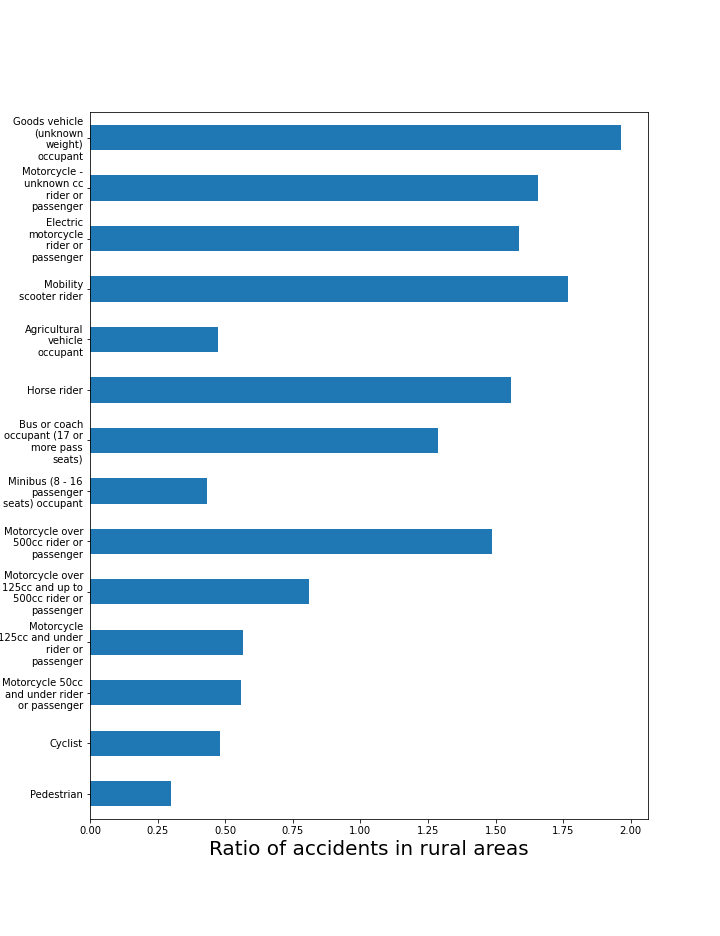
\includegraphics[width=0.70\textwidth]{casualty_rural}
\caption{Ratio of accidents in rural areas to all areas by type of vehicle.}
\label{vehicle-rural}
\end{figure}


This could be due to motorcyclists choosing to ride in more rural areas for recreation, **CITE**, lending to a significant increase in accidents.

\newpage

\subsubsection{Sunrise \& Sunset}

The hypothesis to be tested was that the ratio of average number of accidents per day in darkness would be higher than that in daylight for the same time delta over the entire year. 
As can be seen in figure \ref{sunrise-sunset}, the period tested for sunrise was between 7:00am and 8:00am, and for sunset between 8:30pm and 9:30pm.

\begin{figure}[h]
\centering     %%% not \center
\subfigure[Sunrise times throughout the year.]{\label{fig:sunrise}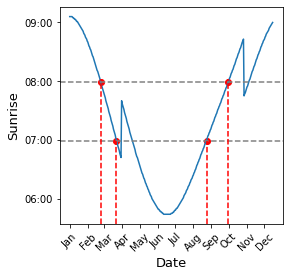
\includegraphics[width=0.45\textwidth]{sunrise_with_lines}}
\subfigure[Sunset times throughout the year.]{\label{fig:sunset}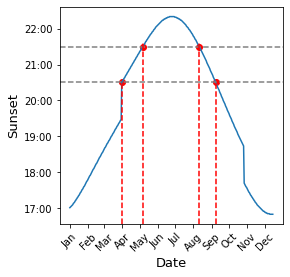
\includegraphics[width=0.45\textwidth]{sunset_with_lines}}
\caption{Sunrise and sunset throughout the year.}
\label{sunrise-sunset}
\end{figure}

To simplify the problem, The dates for which there were days of daylight and darkness in the specified time period were not included. Graphically, this means, for example on figure \ref{fig:sunrise}, that only dates were analysed to the left and right of the outermost red dashed lines, as well as the dates included between the inner lines.

It was found that there was a total of 2988 accidents between 7:00am and 8:00am across the year, 1367 of which occurred during 155 days daylight, and 1621 occurring in 146 days of darkness. This leads to an average number of accidents per day in daylight of 8.82, and 11.10 in darkness. Hence, there is a 26\% increase in accidents during darkness during the hours of 7:00am  to 8:00am.

An equivalent analysis was done for the hours of 8:30pm to 9:30pm. A total of 2143 accidents occurred, 424 of which were during 58 days of daylight, and the remaining 1719 accidents occurred during 204 days of darkness. The average number of accidents per day in daylight for this time period is 7.31, compared to 8.43 in darkness. This leads to a 15\% increase in accidents during darkness during the hour of 8:30pm to 9:30pm.

\subsubsection{Accidents at Premier League Football Matches}

A test case was first carried out for the football match taking place at Old Trafford on Sunday 24th February 2019. Considering any accident within five kilometres of the stadium as being connected to the event, the accident count was compared against the number of accidents in this region every other Sunday during the year. On the day of the match, the number of accidents was 1.77 standard deviations from the mean. This was taken to be significant and worthy of further investigation.

Taking the premier league fixtures of 2019 \parencite{fixtures}, along with the coordinates of every premier league club stadium \parencite{stadiums}, the previous process was done iteratively for a total of 126 football matches during the year at 15 unique stadiums.

\begin{figure}[h]
\centering     %%% not \center
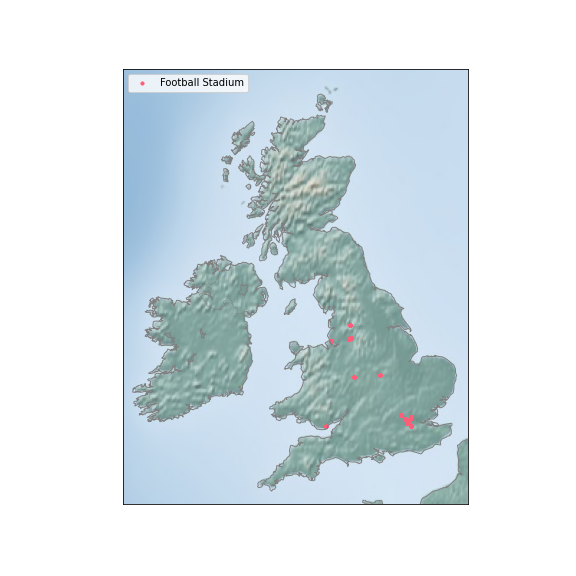
\includegraphics[width=0.70\textwidth]{stadiums}
\caption{Premiere League footaball stadiums analysed.}
\end{figure}

When summarised for every match, the z-score appears to be only 0.05 standard deviations from the average number of accidents. Although there is a significant difference in the number of accidents for different stadiums, on average the analysis implies that there is not a statistically significant rise in the number of accidents on the day of a football match compared to the typical same day of the week in the region.

The table above (figure \ref{football}) shows the summary statistics for premier league football matches. The \textit{Accidents 1} column shows the average number of accidents in the area of the stadium on days when there is a match, and the \textit{Accidents 2} column shows the average number of accidents on the same day of the week when there is not a match being played.


\begin{figure}
    \centering
    \begin{tabular}{|l|l|l|l|}
    \hline
        Stadium & Accidents 1 & Accidents 2 & z-score \\ \hline
        Anfield & 3.0 & 3.6 & -0.12 \\ \hline
        Cardiff City & 1.9 & 1.8 & 0.47 \\ \hline
        Craven Cottage & 16.1 & 16.4 & -0.08 \\ \hline
        Emirates & 21.6 & 21.5 & -0.01 \\ \hline
        Etihad & 3.8 & 5.2 & -0.56 \\ \hline
        Goodison Park & 3.3 & 3.5 & 0.01 \\ \hline
        King Power & 1.7 & 1.9 & 0.34 \\ \hline
        Molineux & 2.2 & 2.9 & -0.29 \\ \hline
        Old Trafford & 4.1 & 4.2 & -0.04 \\ \hline
        Selhurst Park & 14.2 & 11.7 & 0.63 \\ \hline
        Stamford Bridge & 17.1 & 19.9 & -0.47 \\ \hline
        Tottenham Hotspur & 16.4 & 16.5 & -0.0 \\ \hline
        Turf Moor & 0.0 & 1.0 & 0.0 \\ \hline
        Vicarage Road & 0.8 & 2.0 & -0.23 \\ \hline
        Wembley & 9.2 & 12.7 & -0.86 \\ \hline
    \end{tabular}
    \caption{Summary statistics for accidents surrounding Premiere League football stadiums.}
    \label{football}
\end{figure}


\section{Predictive Model}

% introduction

A statistical model was developed in order to predict the conditions under which accidents are most likely to occur in, as well as severity of injuries sustained.
The purpose of developing such a model is to be able to predict when an accident will occur, in order to aid in providing recommendations.

% assumptions

The author assumes that the subset of all data samples that does not contain a single unknown value in the initial predictors of interest is sufficient for training the model. After doing so there was 39,462 samples, 36.27\% of the original data set. A second assumption made was that the nominal, ordinal and binary categorical predictors could all be treated equivalently during the feature selection process.

% feature selection

In order to choose the most suitable features on which to train the model, all the features that seemed to be of value were joined into a single data set. Categorical features were evaluated according to a $\chi^{2}$ hypothesis test CITE, and numerical features according to ANOVA .

% sampling methods

The data was heavily imbalanced on accident severity, on the order of 50:10:1 for slight, serious and fatal injuries respectively. In order to accommodate for this imbalance, an auxiliary data set was produced by oversampling the minority class by using the SMOTE augmentation technique CITE. This provided a balanced set on which the model could be trained.

% models tested

A host of classification models were evaluated by cross-validation on a repeated stratified k-fold of the samples.

Decision tree based models were the by far the most accurate models employed, with the greatest accuracy coming from a stacked model.

\begin{figure}[h]
\centering     %%% not \center
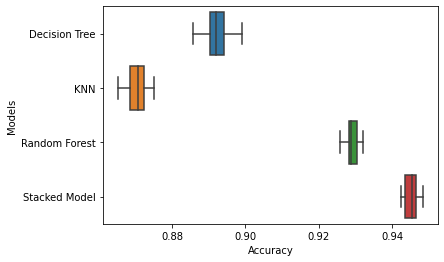
\includegraphics[width=0.80\textwidth]{model_plot}
\caption{Accuracy of models evaluated using cross-validation.}
\label{models}
\end{figure}

As can be seen in figure \ref{models}, a stacked model achieved 95\% accuracy during the cross-validation process. 

However, it should be noted that when the model was later trained on the original dataset, that the accuracy regressed to 87\%.

\section{Predictions}

The author makes the following recommendations based on the analysis delivered.
\begin{itemize}
\item To increase awareness about the dangers of traffic accidents for bicyclers, targeting both the cyclist and the driver.
\item To increase awareness of the dangers of high speed motorcycle use in rural areas, along the lines of **think bikee**. 
\item To consider better lighting conditions during the early hours of the morning and late at night depending on the time of year.
\item To further investigate the reasons why there is a relative increase in accidents involving taxis during the early hours of the morning. This could suggest that overworking and tiredness is playing a key role.
\end{itemize}

\printbibliography

\end{document}